% File : explain_algorithm.tex
% Description: this pdf file explains the Numerov algorithm that has been used in the Numerov file
% Created : august 3 2017
%

\documentclass[12pt]{article}

\usepackage[utf8]{inputenc}
\usepackage[T1]{fontenc}
\usepackage[francais]{babel}
\usepackage{graphicx}
\usepackage{caption}
\usepackage{amsmath}
\usepackage{vmargin}
\usepackage{hyperref}
\usepackage{array}


%%%%%%%%%%%%
% Document %
%%%%%%%%%%%%

\begin{document}

\tableofcontents
\pagebreak


\section{Numerov method}
The Numerov method is a general numerical method to solve second order differential equation of the form

\begin{equation}
\frac{d^2y}{dx^2}+g(x)y(x)+s(x) = 0
\label{NumerovDifEquation}
\end{equation}

where g (x) and s (x) are continuous function on the domain [a,b]. To solve this eaution we will need to solve this problem as a boundary value problem: y (a) and y (b) are known. At this point,
the first thing we need to do is to discretize the interval [a,b] using equally spaced points. Let's say that we fix the distance between each point as h, then we optain a dicrete domain as 
illustrated in figure (1) below.

\begin{figure}[h!]
\centering
\label{interval}
\fbox{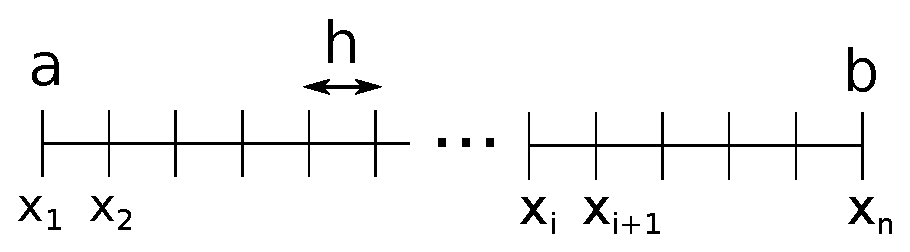
\includegraphics[width=360pt]{interval.eps}}
\caption{The new one dimensional interval after discretization}
\end{figure} 

Then the solution y(x) is also obtain as a discrete set of point for each $x_i$. This means that we now have $y(x)=y(x_i)=y_i$, and the equation is then 

\begin{equation}
\frac{d^2y_i}{dx^2} +g_i(x)y_i(x)+s_i(x) = 0
\label{NumerovEqDiscrete}
\end{equation}

Then if we develop the taylor serie for $y_i$ around $x+h$ we have:

\begin{equation}
y(x+h) = y(x) + hy'(x) + \frac{h^2}{2}y''(x) + \frac{h^3}{6}y^{(3)}(x) + \frac{h^4}{24}y^{4}(x) + \frac{h^5}y^{5}(x) + \cdots
\label{TaylorPlush}
\end{equation}

Similarly for the expansion around $x-h$:

\begin{equation}
y(x+h) = y(x) - hy'(x) + \frac{h^2}{2}y''(x) - \frac{h^3}{6}y^{(3)}(x) + \frac{h^4}{24}y^{4}(x) - \frac{h^5}y^{5}(x) + \cdots
\label{Taylor-h}
\end{equation}

Then by adding equation~\ref{TaylorPlush} and~\ref{Taylor-h}, we obtain 

\begin{equation}
y(x+h) + y(x-h) = 2y(x) + h^2y''(x) + \frac{h^4}{12}y^{4}(x) + O(h^6)
\label{AddingEq}
\end{equation}



\section{Application to the Schödinger equation}

In this script the Numerov method is used to solve the one-dimensionnal time-independant Schrödinger equation. 
The one-dimensional time-independant Scrödinger equation is 
\begin{equation}
-\frac{\hbar^2}{2m}\frac{d^2\psi}{dx^2} + V(x)\psi(x) = E\psi(x)
\label{SchrodEq}
\end{equation}

where $\psi(x)$ is the wavefunction, V (x) the potential energy, $m$ the mass and $\hbar$ the reduced Planck constant. This formula would be hard to compute because of the very small values
of $\hbar$ and $m$ ($\hbar = 1.05457 \cdot 10^{-34}$ and $m_e = 9.11\cdot10^{-31}$), so to avoid dealing with these quantities we use the atomic unit system. In this system, the value of the four
following fundamentals physical constants are unity:  the reduced Planck constant $\hbar$, the elementary charge $e$, the electron mass $m_e$ and Coulomb's constant $k_e = \frac{1}{4\pi\epsilon_0}$.
So in this unit system, Schrödinger's equation is simply:



\section{Algorithm to solve the Schrodinger equation}



\section{More details about the implemented algorithm}



\end{document}
